\sloppy
\documentclass[14pt,a4paper,oneside]{extarticle}	% Размер основного шрифта и формата листа
\usepackage{xltxtra}						% Используется для вывода логотипа XeLaTeX
\usepackage{xunicode}						% Кодировка документа
\usepackage{polyglossia}					% Загружает пакет многоязыковой верстки
\newfontfamily\russianfont{Book Antiqua}
%\setmainfont{Liberation Serif}						% Основной шрифт текста
\setmainfont{Book Antiqua}
\setdefaultlanguage{russian}				% Основной язык текста
\setotherlanguage{english}					% Дополнительный язык текста
\linespread{1}							% Межстрочный интервал выбран полуторным
\usepackage[left=2.5cm,
right=1.5cm,vmargin=2.5cm]{geometry} % Отступы по краям листа
\bibliographystyle{ugost2008}

\usepackage{xcolor}
\usepackage{hyperref}
% Цвета для гиперссылок
\definecolor{linkcolor}{HTML}{359B08} % цвет ссылок
\definecolor{urlcolor}{HTML}{799B03} % цвет гиперссылок
\hypersetup{pdfstartview=FitH,  linkcolor=linkcolor,urlcolor=urlcolor, colorlinks=true}

%---------------------------%
%---- Пакеты расширений ----%
%---------------------------%
\usepackage{xcolor}
\usepackage{hyperref}
% Цвета для гиперссылок
\definecolor{linkcolor}{HTML}{359B08} % цвет ссылок
\definecolor{urlcolor}{HTML}{799B03} % цвет гиперссылок
\hypersetup{pdfstartview=FitH,  linkcolor=linkcolor,urlcolor=urlcolor, colorlinks=true}


\usepackage{verbatim,indentfirst}
\usepackage{cite,enumerate,float}
\usepackage{amsmath,amssymb,amsthm,amsfonts}

%---------------------------%
%--- Вставка иллюстраций ---%
%---------------------------%
\usepackage{graphicx}
\usepackage{subfigure}
%\graphicspath{{Images/}}
\usepackage{fontspec}

\begin{document}
%	\pagestyle{empty} %  выключаенм нумерацию
%\setcounter{page}{3}% Нумерация начинается с третьей страницы
%\renewcommand{\contentsname}{\center{Содержание}}
%\tableofcontents

\begin{center}
	%\addcontentsline{toc}{section}{Опыт 9. Закон Гука}
	\subsection*{Закон Гука}
\end{center}

\begin{figure}[H] 
	\centering 
	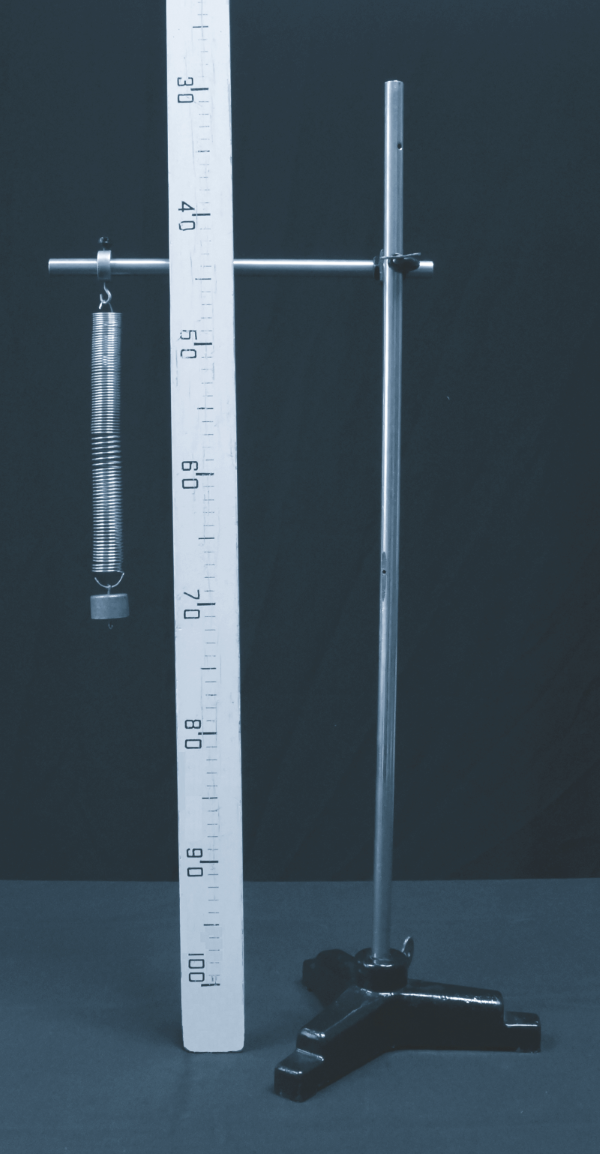
\includegraphics[width=0.4\linewidth]{Hooke-1.png}
	\caption{Демонстрация закона Гука при упругих деформациях}
	\label{Hooke-1}
\end{figure}

\subsection*{\underline{Оборудование:}}

\begin{enumerate}
	\item Набор грузов равной массы (по 100 г каждый)
	\item Пружина
	\item Демонстрационная линейка
	\item Штатив
\end{enumerate}

\newpage
\subsection*{\underline{Основные определения:}}

Закон Гука выражает основной закон между напряженным состоянием и деформацией упругого тела. 
Установлен английским физиком Р. Гуком в 1660 г. для простейшего случая растяжения или сжатия стержня и сформулирован в следующем виде:
 
\begin{flushleft}
	\textit{абсолютное удлинение (укорочение)} $ \Delta l $ \textit{цилиндрического стержня прямо пропорционально растягивающей (сжимающей) силе} $ f $,\textit{т.е.} $ \Delta l \sim lf/ES$, \textit{где} \textit{l} — \textit{длина стержня,} \textit{S} — \textit{площадь его поперечного сечения,} \textit{Е} — \textit{модуль продольной упругости, являющийся механической характеристикой (константой) материала}. 
\end{flushleft}

При малых деформациях, когда величина растяжения или сжатия много меньше размеров стержня, сила упругости пропорциональна деформации тела и направлена в сторону, противоположную направлению перемещения частиц тела при деформации: 
\begin{equation}\label{Hooke-1eq1}
f = –k\Delta l.
\end{equation}

Это соотношение выражает экспериментально установленный закон Гука. 
Коэффициент \textit{k} называется жесткостью тела и зависит от модуля упругости материала пружины и от ее 
геометрических размеров. 

Особенности поведения тела под действием внешних механических нагрузок и возможности практического применения материалов для различных нужд полностью определяются значениями 
модулей упругости (всестороннего сжатия, Юнга и др.) и расположением точек пределов упругости и прочности. 
Такие материалы, как сталь и титан, обладают высокими значениями модулей упругости, высокими пределами упругости и прочности.
Это позволяет широко использовать их в различных сооружениях и машинах. 

Свинец и воск обладают низким пределом упругости и намного 
более высоким пределом прочности.
Это — мягкие пластичные тела, которые начинают течь уже при небольших деформациях. 

У стекла и кварца предел прочности лежит в области очень малых деформаций и ниже предела упругости.
Это — хрупкие тела, которые могут испытывать только очень небольшие упругие деформации и затем разрушаются. 

В технике часто применяются спиралеобразные пружины.
При растяжении или сжатии пружин возникают упругие силы, которые также подчиняются закону Гука.
В пределах применимости закона Гука пружины способны сильно изменять свою длину.
Поэтому их часто используют для измерения сил. 
Пружину, растяжение которой проградуировано в единицах силы, называют динамометром.
Следует иметь в виду, что при растяжении или сжатии пружины в ее витках возникают сложные деформации кручения и изгиба.

Соотношение (\ref{Hooke-1eq1}) оказывается справедливым для всех упругих пружин и тел.
Поэтому для расчета внешних действий упругих пружин закон Гука можно сформулировать так:
\textit{\begin{flushleft}
		сила действия упругой пружины пропорциональна растяжению 
(сжатию) этой пружины.
\end{flushleft}} 

\subsection*{\underline{Краткое описание:}}

С целью демонстрации проявления закона Гука на штативе закрепляются пружина с грузом и линейка.
Опыт заключается в измерении положения груза, подвешенного за пружину.
В первую очередь записывается начальное положение конца ненагруженой пружины — $x_0 $.
Затем за нижний конец пружины подвешивается груз массой 100 г и в таблицу записывается новая координата — $x_1 $.
Постепенно пружину необходимо нагрузить четырьмя или пятью грузами и записать все результаты в виде таблицы.
После этого можно построить график зависимости силы упругости (численно равна силе тяжести нагрузки, создаваемой грузами) от величины удлинения пружины $x_1 - x_0$.

\begin{figure}[H] 
	\centering 	
	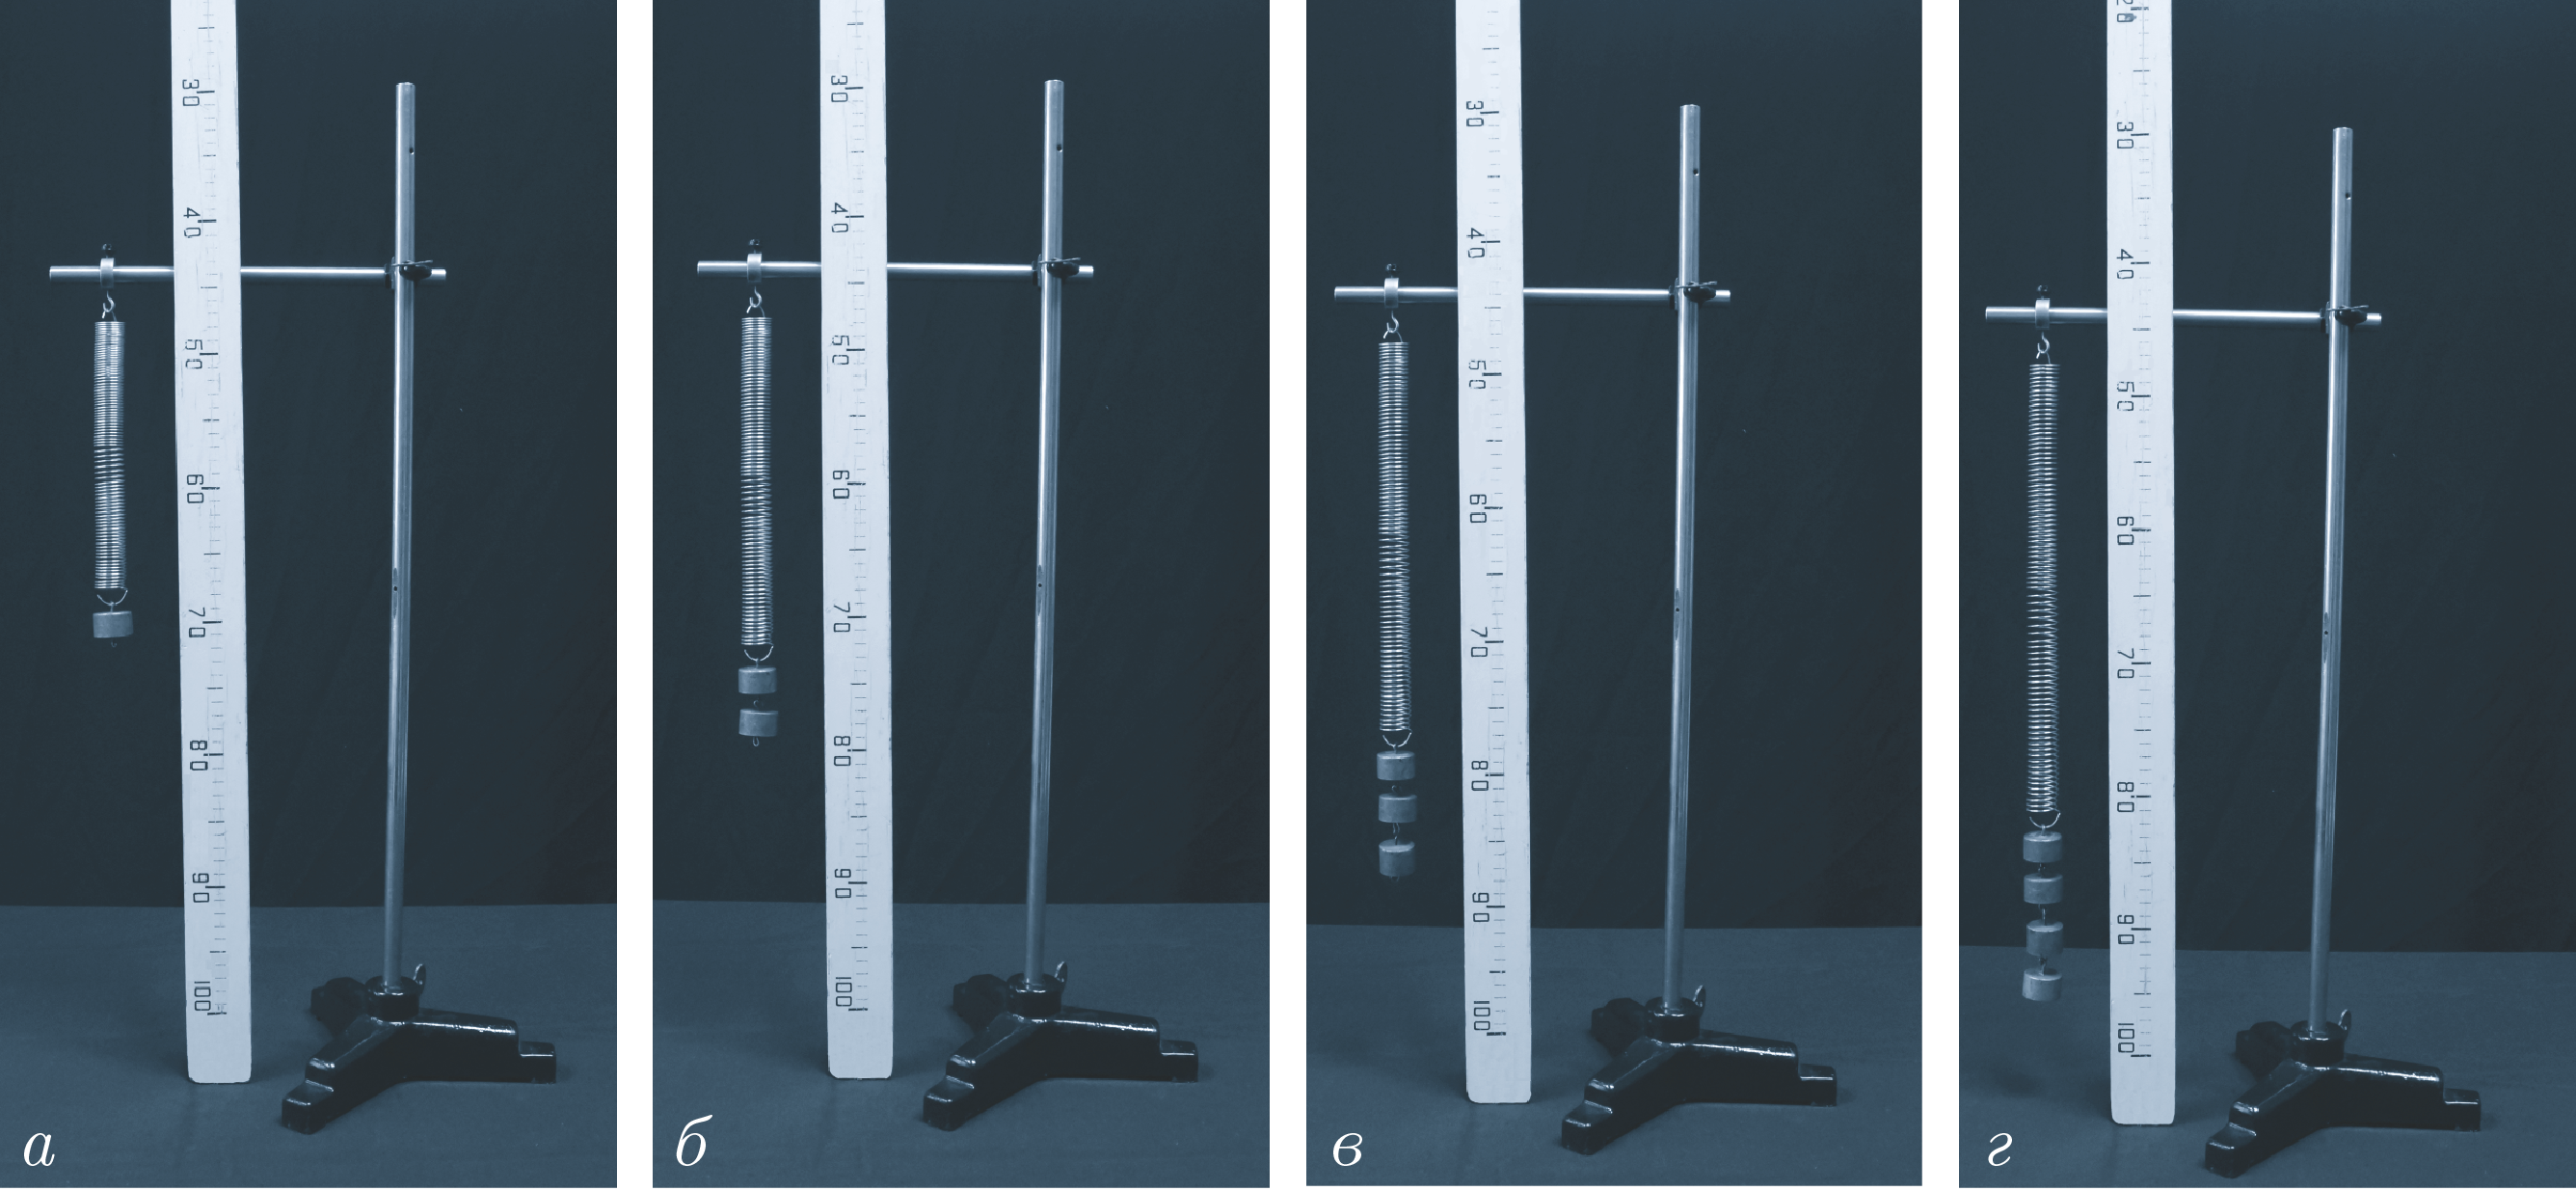
\includegraphics[width=0.9\linewidth]{Hooke-2.png}
	\caption{Демонстрация растяжения пружины под действием силы тяжести со стороны одного, двух, трех и четырех грузов соответственно}
	\label{Hooke-2}
\end{figure}

Таким образом, измеряя удлинения $ \Delta x $, которые будет приобретать пружина, можно убедиться в том, что 
они растут пропорционально напряжениям, которые создаются в пружине подвешенными грузами. 

\newpage
\subsection*{\underline{Теория:}}

Рассмотрим деформацию (растяжение) упругой пружины, один из концов которой жестко закреплен, а снизу к пружине повешен груз массой \textit{m} (рис.\ref{Hooke-3}).
Под действием силы тяжести (веса) со стороны груза пружина деформируется (при растяжении ее длина увеличится на величину $ \Delta x $).
При этом в пружине возникнет сила, противодействующая деформации — сила упругости $ f $.

\begin{figure}[H] 
	\centering 	
	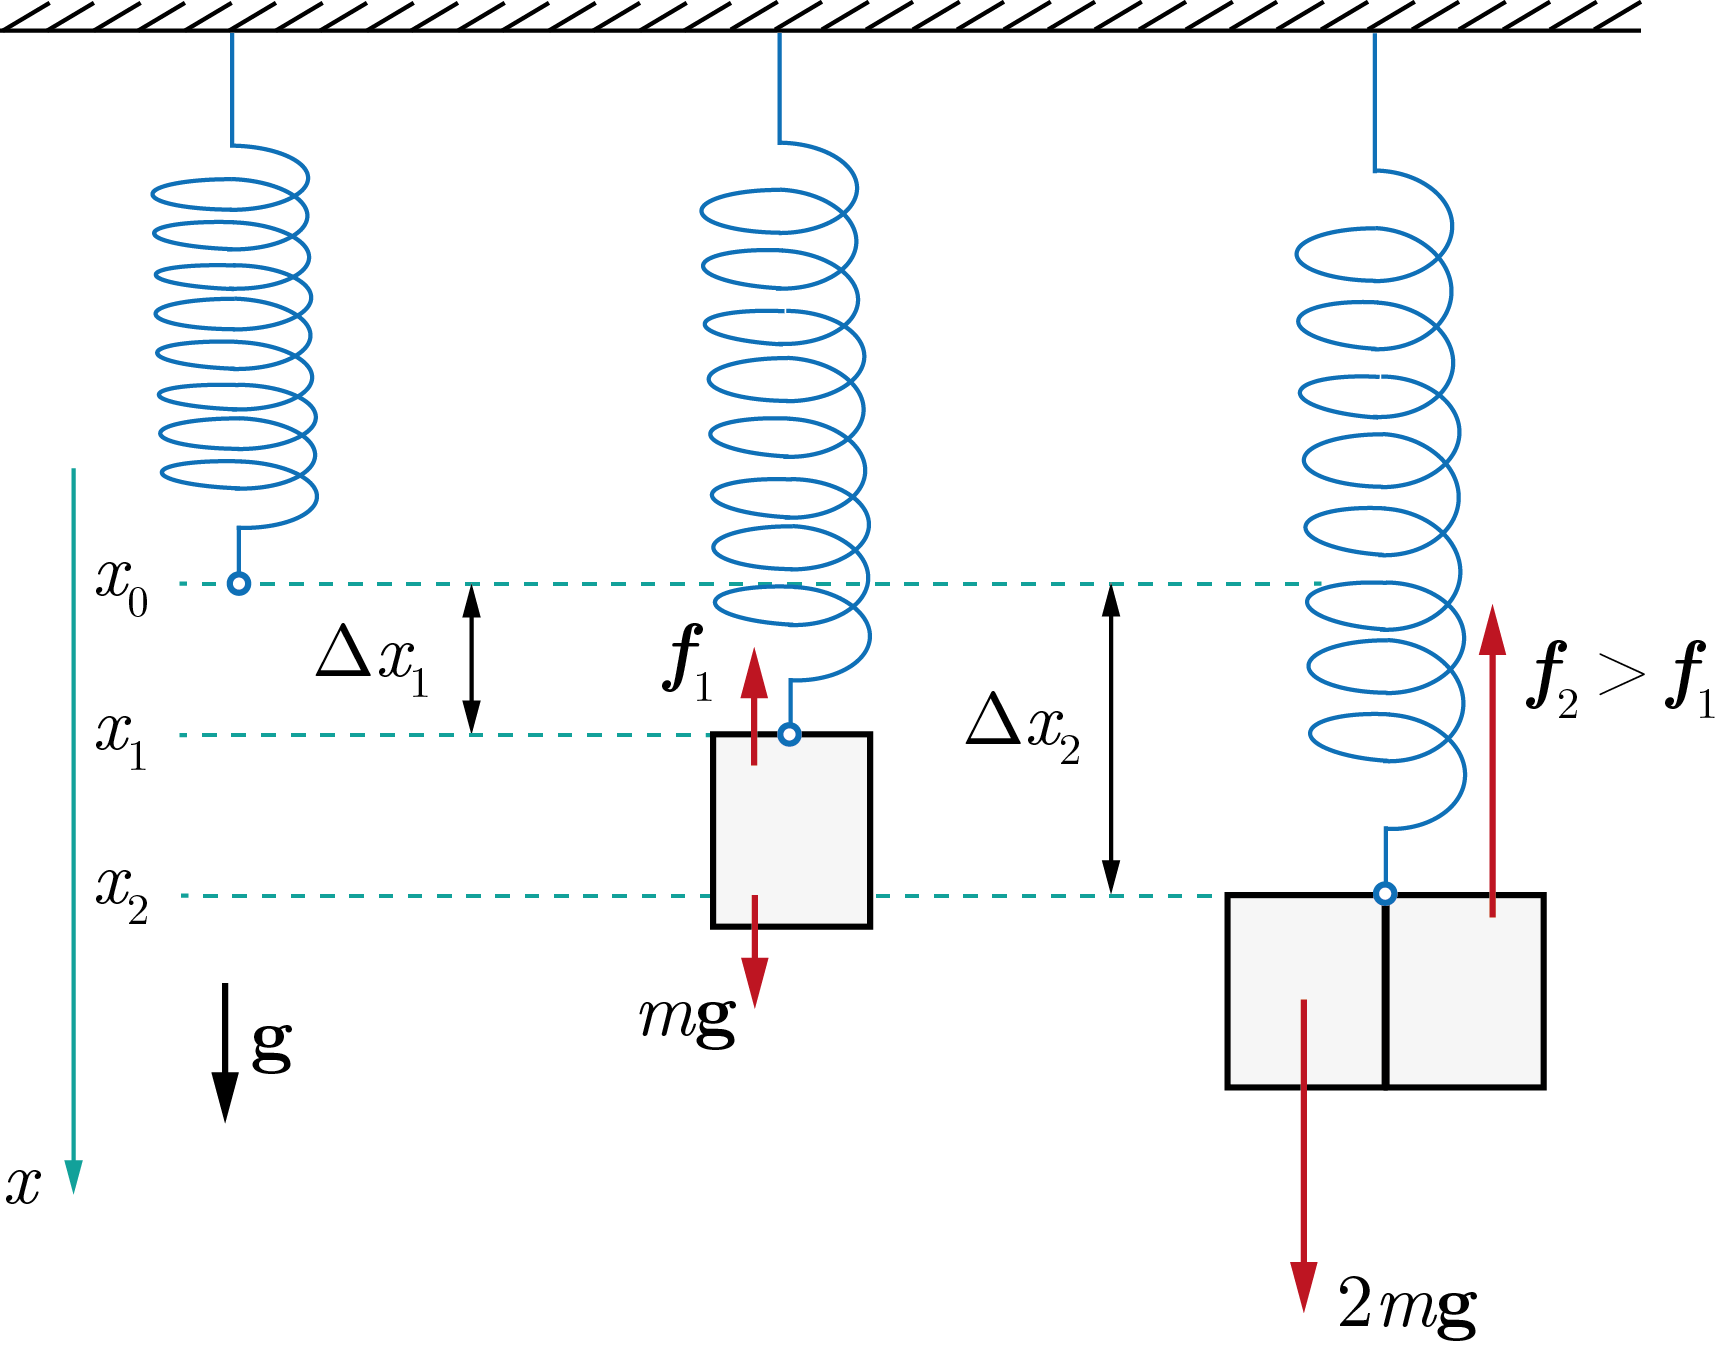
\includegraphics[width=0.6\linewidth]{Hooke-3.png}
	\caption{Схема растяжения пружины, показывающая как ее удлинение зависит от массы подвешиваемого груза}
	\label{Hooke-3}
\end{figure}

Эта сила будет действовать на груз, который и вызывает деформацию.
Если движение в системе не происходит, пружина и груз находятся в покое ($ \textbf{a}=0 $), то сила упругости растянутой пружины уравновесит силу тяжести:
\begin{equation}\label{Hooke-1eq2}
0=m\textbf{g}+ \textit{\textbf{f}}
\end{equation}
или в проекции на ось \textit{x}:
\begin{equation}
f=mg.
\end{equation}

Используя закон Гука, можно получить:
\begin{equation}\label{Hooke-1eq3}
k\Delta x=mg
\end{equation}
или
\begin{equation}\label{Hooke-1eq4}
\Delta x = g\frac mk.
\end{equation}

Отсюда следует, что удлинение пружины прямо пропорционально массе повешенного к ней груза и обратно пропорционально ее жесткости.

\end{document}